\problemname{Berguppdelning}

\noindent Danskarna är avundsjuka på att alla andra länder har så mycket bättre skidbackar. 
Frågan har tagits hela vägen till EU-domstol, 
och det har beslutats att man ska rita om landsgränserna i Europa så att fördelningen 
av skidbackar blir så jämn som möjligt. Europa kan modelleras som ett rutnät av storlek $R \cdot C$,
där det till varje ruta hör ett tal $m_{ij}$ som beskriver hur många berg det finns där.
Ett land består av en sammanhängande mängd rutor,
där det totala antalet berg i landet dividerat med landets
yta avgör hur trevligt det är att åka skidor där.
Hjälp danskarna att dela upp Europas $N$ länder så att 
bergen är fördelade så jämnt som möjligt, relativt till ländernas yta!


\section*{Indata}
Den första raden innehåller ett heltal $T$, numret på det testfall som körs.
Den andra raden innehåller tre heltal 
$R, C$ ($2 \le R \cdot C \le 10^6$), $N$ ($1 \le N \le 10^5$), 
antalet rader respektive kolumner i rutnätet,
och antalet länder.
Därefter följer $R$ rader, en för varje rad i rutnätet. 
Varje rad innehåller $C$ tal. På rad $i$, kolumn $j$ 
står talet $m_{ij}$ ($0 \leq m_{ij} \leq 1000$), 
antalet berg på motsvarande plats i rutnätet.

\section*{Utdata}
Skriv ut $R$ rader med $C$ tal vardera, där varje tal motsvarar vilket land som äger rutan efter uppdelningen. 
Varje land identifieras med ett tal $0 \leq x < n$.

\section*{Poängsättning}
Din lösning kommer att testas på 10 testfall, 
där varje fall ger upp till 10 poäng. 
Låt $a_k$ vara mängden berg i land $k$ dividerat med antalet rutor i landet, 
och låt $\bar{a}$ vara det totala antalet berg dividerat med det totala antalet rutor i hela rutnätet.
Du vill minimera värdet av uttrycket 


\[
S = \sum_{k=1}^{n}{(a_k - \bar{a})^2}. 
\]

\noindent Om $S = 0$ får din lösning 10 poäng i testfallet. 
Annars bestäms din poäng enligt uttrycket 

\[
10 \cdot \texttt{max}(1, \frac{S_D}{S}),
\]

\noindent där $S_D$ är vad domarlösningen uppnådde på samma testfall. 


\noindent
\begin{tabular}{| l | l | p{12cm} |}
  \hline
  \textbf{Grupp} & \textbf{Poäng} & \textbf{Gränser} \\ \hline
  $1$    & $10$      & $R = C = N = 10$ \\ \hline
  $2$    & $10$      & $R = 1$, $C = 100000$, $N = 1000$ \\ \hline
  $3$    & $10$      & $R = 2$, $C = 10000$, $N = 1000$ \\ \hline
  $4$    & $10$      & $R = C = 200$, $N = 40$, $m_{ij} = 0$ eller $m_{ij} = 1$ för alla $i$, $j$ \\ \hline
  $5$    & $10$      & $R = C = 50$, $N = 250$ \\ \hline
  $6$    & $10$      & $R = C = 200$, $N = 2$ \\ \hline
  $7$    & $10$      & $R = C = 200$, $N = 400$ \\ \hline
  $8$    & $10$      & $R = C = 400$, $N = 16000$ \\ \hline
  $9$    & $10$      & $R = C = 400$, $N = 1600$ \\ \hline
  $10$    & $10$      & $R = C = 400$, $N = 1600$ \\ \hline
\end{tabular}

\section*{Förklaring av exempelfall 1}
\begin{figure}[!h]
  \centering
  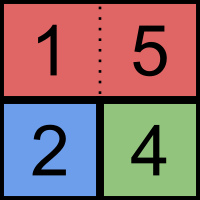
\includegraphics[width=2cm]{sample1.png}
  \quad
  \caption{Uppdelningen av länder i exempelfall 1.}
\end{figure}

\noindent I det första exempelfallet är $\bar{a} = \frac{1 + 5 + 2 + 4}{4} = 3$. Medelvärderna är 3 för det röda landet, 2 för det blåa och 4 för det gröna. Detta ger $S = 2$.

\section*{Förklaring av exempelfall 2}
\begin{figure}[!h]
  \centering
  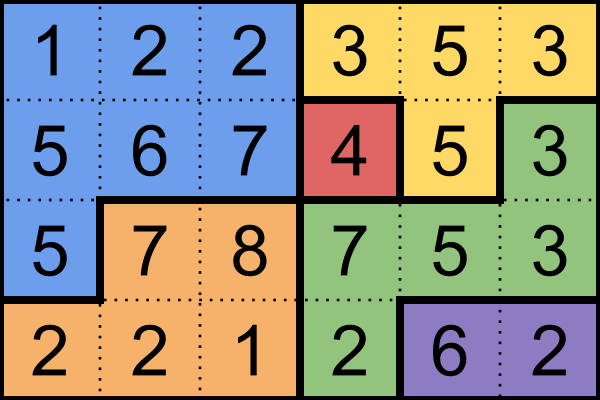
\includegraphics[width=5cm]{sample2.png}
  \quad
  \caption{Uppdelningen av länder i exempelfall 1.}
\end{figure}

\noindent I det andra exempelfallet är $\bar{a} = 4$. Medelvärdet i varje land är 4. Detta ger $S = 0$, alltså en perfekt lösning.
